\documentclass{phyasgn}
\phyasgn{
  stuname = 姚昊廷,           % 设置学生姓名
  stunum = 22322091,      % 设置学号
  setasgnnum = 7,           % 设置课程次数
  classname = 电磁学,     % 设置课程名称
}

\usepackage{listings}
\usepackage{tikz}
\usepackage{amssymb}
\usepackage{t-angles}
\usepackage{amssymb}
\usepackage{tikz}
%\usepackage{autobreak} 
%\usepackage{fixdif} 
\usetikzlibrary{quotes,angles}
\usetikzlibrary{calc}
\usetikzlibrary{decorations.pathreplacing}
\lstset{numbers=left,basicstyle=\ttfamily,columns=flexible}
\makeatletter
\newcommand{\rmnum}[1]{\romannumeral #1}
\newcommand{\Rmnum}[1]{\expandafter\@slowromancap\romannumeral #1@}
\makeatother


\begin{document}
{\zihao{5}\heiti\color{red} 4-3}
\begin{sol}
    \begin{figure}[!h]
        \begin{tikzpicture}
        
            \draw (-5,5) rectangle (5,4.9);
            \draw (-5,4.9) rectangle (5,3);
            \draw (-5,3) rectangle (5,0);
            \draw (-5,0) rectangle (5,-0.1);
            \node at(0,3.5){$\varepsilon_1$};
            \node at(0,1.5){$\varepsilon_2$};
            \draw (-1,4.95) rectangle (1,4);
            \draw (-1,-0.05) rectangle (1,1);
            \node at(0,4.5){$\Rmnum{1}$};
            \node at(0,0.5){$\Rmnum{2}$};
        \end{tikzpicture}
    \end{figure}\par
(1)设上极板所带电荷面密度为$\sigma$,取如图所示二高斯面可知
$D=\sigma$,则
$$\begin{aligned}
    E_1&=\frac{D}{\varepsilon_0\varepsilon_1}\\
    E_2&=\frac{D}{\varepsilon_0\varepsilon_2}
\end{aligned}$$
又
$$
E_1d_1+E_2d_2=U
$$
解得$\sigma=4.66\times 10^{-5}\mathrm{C/m^2}$
故
$$\begin{aligned}
    P_1&=\frac{\varepsilon_1-1}{\varepsilon_1}\sigma=3.7\times 10^{-5}\mathrm{C/m^2}\\
    P_1&=\frac{\varepsilon_2-1}{\varepsilon_2}\sigma=1.6\times 10^{-5}\mathrm{C/m^2}
\end{aligned}$$\par
(2)$$U=E_2d_2=7.9\times 10^3\mathrm{V}$$
\end{sol}\par

{\zihao{5}\heiti\color{red} 4-6}
\begin{sol}
由对称性知,两平行板之间电场应垂直于导体板,亦即互相平行,故其中间为匀强电场
设场强为$E$故有
$$\begin{aligned}
    \sigma_1&=\varepsilon_0\varepsilon_1E\\
    \sigma_2&=\varepsilon_0\varepsilon_2E
\end{aligned}$$
又$Q=\sigma_1S_1+\sigma_2S_2,U=Ed$,故电容为
$$\begin{aligned}
    C&=\frac{Q}{U}\\
    &=\frac{(\varepsilon_1S_1+\varepsilon_2S_2)\varepsilon_0}{d}
\end{aligned}$$
\end{sol}\par

{\zihao{5}\heiti\color{red} 4-9}
\begin{sol}
(1)$$E=\left\{\begin{matrix}
    \frac{Q}{4\pi\varepsilon \varepsilon _0r^2} &R<r<R^{\prime} \\
   \frac{Q}{4\pi \varepsilon _0r^2}&r<R^{\prime}
  \end{matrix}\right.$$
(2)$$U=\left\{\begin{matrix}
    &\int_r^{R^{\prime }}E\d r+\int_{R^{\prime }}^\infty E\d r=\frac{Q}{4\pi\varepsilon \varepsilon _0}(\frac{1}{r}+\frac{\varepsilon -1}{R^{\prime }}  ) &R<r<R^{\prime} \\
  &\\
  &\int_{r}^\infty E\d r=\frac{Q}{4\pi\varepsilon _0r}&r>R^{\prime} 
  \end{matrix}\right.$$
(3)$$U=\frac{Q}{4\pi\varepsilon \varepsilon _0}(\frac{1}{R}+\frac{\varepsilon -1}{R^{\prime }}  ) $$
\end{sol}\par

{\zihao{5}\heiti\color{red} 4-12}
\begin{sol}
$D=\frac{Q}{4\pi r^2}$故
$$\begin{aligned}
    E_1&=\frac{D}{\varepsilon_1\varepsilon_0}\\
    E_2&=\frac{D}{\varepsilon_2\varepsilon_0}
\end{aligned}$$
故两极板间电势差为

$$U=\int_{R_1}^RE_1\d r+\int_R^{R_2}E_2\d r=\frac{Q}{4\pi\varepsilon_0}\left [  (\frac{1}{\varepsilon_1R_1}-\frac{1}{\varepsilon_1R})+(\frac{1}{\varepsilon_2R}-\frac{1}{\varepsilon_2R_2})\right ] $$
则电容为
$$C=\frac{Q}{U}=\frac{4\pi\varepsilon_0}{(\frac{1}{\varepsilon_1R_1}-\frac{1}{\varepsilon_1R})+(\frac{1}{\varepsilon_2R}-\frac{1}{\varepsilon_2R_2})}$$
(2)$$\begin{aligned}
    \sigma(R_1)&=P_1=\frac{(\varepsilon_1-1)Q}{   4\pi\varepsilon_1R_1^2}\\
    \sigma(R)&=\frac{(\varepsilon_2-1)Q}{4\pi\varepsilon_2R^2}-\frac{(\varepsilon_1-1)Q}{4\pi\varepsilon_1R^2}=\frac{(\varepsilon_2-\varepsilon_1)Q}{4\pi\varepsilon_1\varepsilon_2R^2}\\
    \sigma(R_2)&=-\frac{(\varepsilon_2-1)Q}{4\pi\varepsilon_2R_2^2}
\end{aligned}$$
\end{sol}\newpage

{\zihao{5}\heiti\color{red} 4-19}
\begin{sol}
\begin{figure}[!h]
    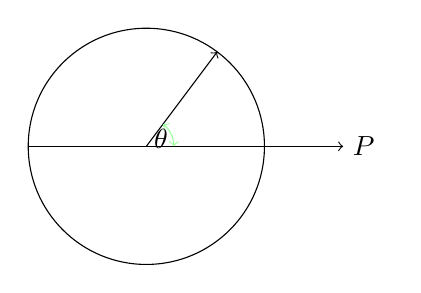
\begin{tikzpicture}
        \coordinate (a) at (1,0);
        \coordinate (b) at (1.8,2.4);
        \coordinate (o) at (0,0);
        \draw[->,scale=0.5] (-3,0) --(5,0)node[right]{$P$};
        \draw[scale=0.5] (0,0) circle (3);
        \draw[->,scale=0.5] (0,0) --(1.8,2.4);
        \pic[scale=0.5]["$\theta$", draw=green!40, <->, angle eccentricity=0.6, angle radius=0.7cm]
    {angle=a--o--b};
    \end{tikzpicture}
\end{figure}\\
    
    轴线处场强由分界面内部和外部电荷共同作用产生,界面内部极化电荷分布在圆柱表面
    可看作多个无限长带电直线叠加,极矩$P=(\varepsilon-1)\varepsilon_0E_0$,则极化
    电荷面密度为$P\cos\theta$,线密度就为$\lambda=P\cos\theta r\d \theta$,又因为
    系统的对称性,故可知何场强方向一定与$P$方向共线则其在轴线处的场强大小为
    $$E=\int_0^{2\pi}\frac{\lambda\cos\theta}{2\pi R\varepsilon_0}=\frac{P}{2\pi\varepsilon_0}\int_0^{2\pi}\cos^2\theta \d\theta=\frac{P}{2\varepsilon_0}=\frac{\varepsilon-1}{2}E_0$$
    又因为该场强与$E_0$方向相反故
    $$E=E_0+\frac{\varepsilon-1}{2}E_0=\frac{\varepsilon+1}{2}E_0$$
    真挖去后不成立,因为极化不再均匀
\end{sol}\par
\end{document}